%! TEX program = xelatex
%! TEX root = ../main.tex
%! TEX encoding = utf-8

%%%%%%%%%%%%%%%%%%%%%%%%%%%%%%%%%%%%%%%%%%%%%%%%%%%%%%%%%%%%%%%%%%%%%%
%
%  哈尔滨工程大学学位论文 XeLaTeX 模版 —— 正文文件 chap04.tex
%
%  版本:1.0.0
%  最后更新:
%  修改者:Leo LiWenhui lwh@hrbeu.edu.cn
%  修订者:
%  编译环境1:Ubuntu 12.04 + TeXLive 2013/2014
%  编译环境2:Windows 7/8  + TeXLive 2013/2014
%
%%%%%%%%%%%%%%%%%%%%%%%%%%%%%%%%%%%%%%%%%%%%%%%%%%%%%%%%%%%%%%%%%%%%%

\chapter{列表}[Table]
\label{chap04}

\section{研究生院的绘表规范}[Requirement of Table]

表应有自明性。表格不加左、右边线。表的编排建议采用国际通行的三线表。表中文字用宋体~5~号字。

每个表格均应有表题(由表序和表名组成)。表序一般按章编排,如第~1~章第一个插表的序号为“表~1.1”等。表序与表名之间空一格,
表名中不允许使用标点符号,表名后不加标点。表题置于表上,硕士学位论文只用中文,博士学位论文用中、英文两种文字居中排写,
中文在上,要求中文用宋体~5~号字,英文用新罗马字体~5~号字。

表头设计应简单明了,尽量不用斜线。表头中可采用化学符号或物理量符号。

全表如用同一单位,则将单位符号移至表头右上角,加圆括号。
表中数据应准确无误,书写清楚。表内文字或数字上、下或左、右相同时,
采用通栏处理方式,不允许用“〃”、“同上”之类的写法。

表内文字说明,起行空一格、转行顶格、句末不加标点。

如某个表需要转页接排,在随后的各页上应重复表的编号。编号后加“(续表)”,表题可省略。续表应重复表头。

\section{普通表格的绘制方法}[General Table]

表格应具有三线表格式,因此需要调用~booktabs~宏包,其标准格式如表~\ref{table1}~所示。
\begin{table}[htbp]
\bicaption[table1]{}{符合研究生院绘图规范的表格}{Table$\!$}{Table in agreement of the standard from graduate school}
\vspace{0.5em}\centering\wuhao
\begin{tabular}{ccccc}
\toprule[1.5pt]
$D$(in) & $P_u$(lbs) & $u_u$(in) & $\beta$ & $G_f$(psi.in)\\
\midrule[1pt]
 5 & 269.8 & 0.000674 & 1.79 & 0.04089\\
10 & 421.0 & 0.001035 & 3.59 & 0.04089\\
20 & 640.2 & 0.001565 & 7.18 & 0.04089\\
\bottomrule[1.5pt]
\end{tabular}
\end{table}

其绘制表格的代码及其说明如下。
\vspace{1em}
\begin{lstlisting}
\begin{table}[htbp]
\bicaption[标签名]{}{中文标题}{Table$\!$}{English caption}
\vspace{0.5em}\centering\wuhao
\begin{tabular}{cc...c}
\toprule[1.5pt]
表头第1个格   & 表头第2个格   & ... & 表头第n个格  \\
\midrule[1pt]
表中数据(1,1) & 表中数据(1,2) & ... & 表中数据(1,n)\\
表中数据(2,1) & 表中数据(2,2) & ... & 表中数据(2,n)\\
...................................................\\
表中数据(m,1) & 表中数据(m,2) & ... & 表中数据(m,n)\\
\bottomrule[1.5pt]
\end{tabular}
\end{table}
\end{lstlisting}

又例如表~\ref{tab:xingxing}展示了太阳系的各行星的位置。
\begin{figure}[htbp]
  \centering
  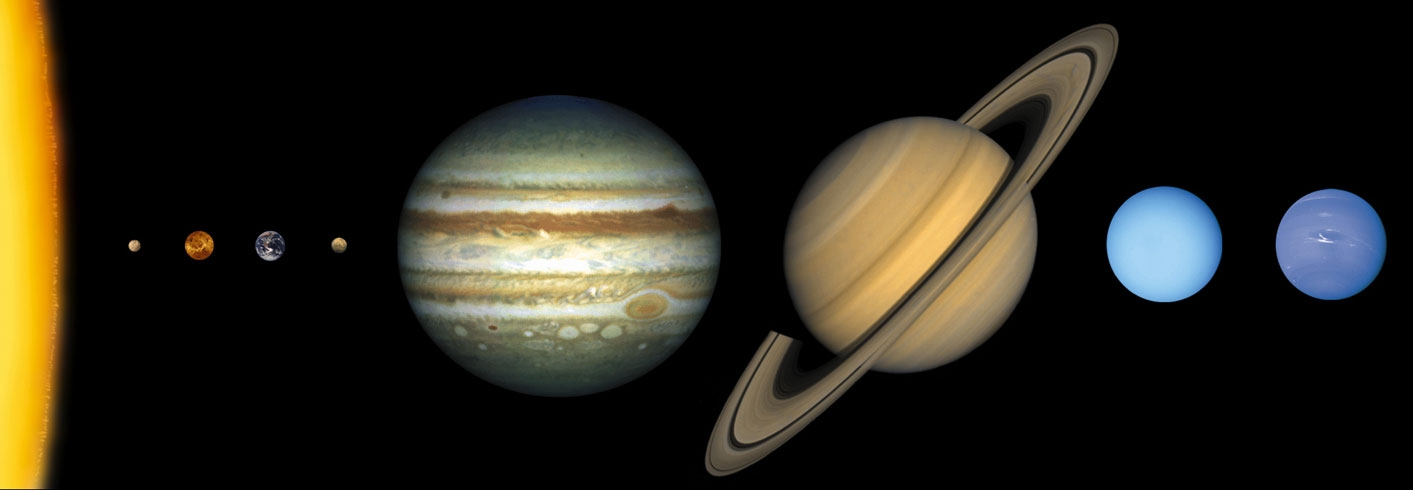
\includegraphics[width=0.9\textwidth{},keepaspectratio]{sun.jpg}
  \bicaption[fig:sun]{太阳系}{最左侧是太阳,向右依序为水星、金星、地球、火星、
    木星、土星、天王星与海王星}{Fig.}{Outward from the Sun, the planets
    are Mercury, Venus, Earth, Mars, Jupiter, Saturn, Uranus and
    Neptune.}
\end{figure}

\begin{table}[htbp]
  \bicaption[tab:xingxing]{行星数据表1}{行星数据表}{Tab.}{Planet}
  \centering
  \vspace{0.2cm}
  \wuhao
  \begin{tabular}{cccc}
    \toprule
    Planet  & Size(Earth=1) & Weight(Earth=1) & Radius  \\
    \midrule
    Mercury & 0.056         & 0.055           & 0.3871  \\
    Venus   & 0.857         & 0.815           & 0.7233  \\
    Earth   & 1.00          & 1.000           & 1.0000  \\
    Mars    & 0.151         & 0.107           & 1.5237  \\
    Jupiter & 1321          & 317.832         & 5.2026  \\
    Saturn  & 755           & 95.16           & 9.5549  \\
    Uranus  & 63            & 14.54           & 19.2184 \\
    Neptune & 58            & 17.15           & 30.1104 \\
    \bottomrule
  \end{tabular}
\end{table}

表~\ref{tab:xingxing}的源代码如下:
\vspace{1em}
\begin{lstlisting}
  \begin{table}[htbp]
    \bicaption[tab:xingxing]{行星数据表1}{行星数据表}{Tab.}{Planet}
    \centering
    \vspace{0.2cm}
    \wuhao
    \begin{tabular}{cccc}
      \toprule
      Planet  & Size(Earth=1) & Weight(Earth=1) & Radius  \\
      \midrule
      Mercury & 0.056         & 0.055           & 0.3871  \\
      Venus   & 0.857         & 0.815           & 0.7233  \\
      Earth   & 1.00          & 1.000           & 1.0000  \\
      Mars    & 0.151         & 0.107           & 1.5237  \\
      Jupiter & 1321          & 317.832         & 5.2026  \\
      Saturn  & 755           & 95.16           & 9.5549  \\
      Uranus  & 63            & 14.54           & 19.2184 \\
      Neptune & 58            & 17.15           & 30.1104 \\
      \bottomrule
    \end{tabular}
  \end{table}
\end{lstlisting}

表格和插图通常需要占据大块空间,所以在文字处理软件中用户经常需要调整它们的
位置。 \texttt{table}环境可以自动完成这样的任务,这种自动调整位置的环境称作
浮动环境 (float)\footnote{下一节里还会介绍插图浮动环境}。table环境是一个将表格嵌入文本的浮动环境。

\texttt{htbp} 选项用来指定表格的理想位置,这几个字母分别代表 here, top,
bottom,float page,也就是就这里、页顶、页尾、浮动页 (专门放浮动环境的单独
页面)。我们可以使用这几个字母的任意组合,四个字母都写上表示放哪里都无所
谓;一般不推荐单独使用\texttt{h},因为 \LaTeX{}自以为它的排版算法是最完美的,不愿意
被束缚手脚。

\verb|\centering| 用来使表格居
中; \verb|\bicaption| 命令设置表格标题, \LaTeX{}会自动给
浮动环境的标题加上编号。

它的官方使用说明为:
\begin{lstlisting}
  \bicaption[label]{ 中文短标题 }{ 中文标题 }{Tab.}{ 英文标题 }
\end{lstlisting}
可选参数~label~用来作为交叉引用链接。例如
表~\ref{tab:xingxing}中的 lable为 tab:xingxing 。这里的标
签一般为英文。中文短标题一般没什么用,可以随意填。最简单就是“表”。

在表格环境中,标题必须位于表格的上方。而在图片环境中,标题的位置必须位于
图片的下方。

tabular 环境提供了最简单的表格功能。它用 \texttt{\&} 来分列,
用 \texttt{\textbackslash{\textbackslash{}}} 来换行;每列可以采用居中、居
左、居右等横向对齐方式,分别用 \texttt{l、c、r} 来表示。

三线表的三条横线就分别
用 \verb|\toprule、 \midrul、\bottomrule| 等命令表示。

\verb|\vspace{0.2cm}| 是用来控制表格标题与表格正文的
垂直间距的,请在插入表格时务必添加。 \verb|\wuhao| 是
用来调整表格内容的行距的。


\subsection{多列三线表}[Three Line Table]

在三线表中,有些列的列头会横跨好几列的数据。一般使
用 \verb|\multicolumn| 命令。它的用法是:
\begin{lstlisting}
  \multicolumn{ 列数}{ 对齐方式 }{ 表格内容 }
\end{lstlisting}

“列数”是指这一列横跨的列数,在表~\ref{tab:linux}是2列,就填“2”;“对
齐方式”从\texttt{lcr}三者中选其一即可,在表~\ref{tab:linux}中是\texttt{c}。“表格
内容”填入自己的内容。一般还会在这一列的下面画一小横线,已示辨识。使
用 \verb|\cmidrule| 命令。在表~\ref{tab:linux}中,由于横跨的是第2列和第3列,
因此 \verb|\cmidrule| 的参数是2-3。

\begin{table}[htbp]
  \bicaption[tab:linux]{不同操作系统下的\LaTeX{}}{ 不同操作系统下的\LaTeX{} }{Tab.}{OS with \LaTeX{}}
  \centering
  \vspace{0.2cm}
  \wuhao
  \begin{tabular}{ccc}
    \toprule
    Test    & \multicolumn{2}{c}{Common Tools} \\
              \cmidrule{2-3}
    OS         & Distribution & Editor  \\
    \midrule
    Windows    & MikTeX       & TexMakerX  \\
    Mac OS     & MacTeX       & TeXShop  \\
    Linux/Unix & TeX Live     & TeXworks  \\
    \bottomrule
  \end{tabular}
\end{table}


\begin{lstlisting}
  \begin{table}[htbp]
    \bicaption[tab:linux]{不同操作系统下的\LaTeX{}}{不同操作系统下的\LaTeX{}}
    {Tab.}{OS with \LaTeX{}}
    \centering
    \vspace{0.2cm}
    \wuhao
    \begin{tabular}{ccc}
      \toprule
      Test    & \multicolumn{2}{c}{Common Tools} \\
                \cmidrule{2-3}
      OS         & Distribution & Editor  \\
      \midrule
      Windows    & MikTeX       & TexMakerX  \\
      Mac OS     & MacTeX       & TeXShop  \\
      Linux/Unix & TeX Live     & TeXworks  \\
      \bottomrule
    \end{tabular}
  \end{table}
\end{lstlisting}

\subsection{多行三线表}[Multiline Table]

既然有多列三线表,多行三线表也是用类似的方法解决。我们把表~\ref{tab:linux} 来改造一下,相对应的,一般使用 \verb|\multirow| 命令。它的用法
是:
\begin{lstlisting}
  \multirow{ 行数 }*{ 表格内容 }
\end{lstlisting}

“行数”是指竖向跨的行数,在表~\ref{tab:unix}中是2行,中间有个星号,表示自然宽度。

\begin{table}[htbp]
  \bicaption[tab:unix]{不同操作系统下的\LaTeX{}}{ 不同操作系统下的\LaTeX{} }{Tab.}{OS with \LaTeX{}}
  \centering
  \vspace{0.2cm}
  \wuhao
  \begin{tabular}{ccc}
    \toprule
    \multirow{2}*{OS} & \multicolumn{2}{c}{Common Tools} \\
                        \cmidrule{2-3}
                      & Distribution & Editor  \\
    \midrule
    Windows          & MikTeX       & TexMakerX  \\
    Mac OS           & MacTeX       & TeXShop  \\
    Linux/Unix       & TeX Live     & TeXworks  \\
    \bottomrule
  \end{tabular}
\end{table}


\begin{lstlisting}
  \begin{table}[htbp]
    \bicaption[tab:unix]{不同操作系统下的\LaTeX{}}{不同操作系统下的\LaTeX{}}
    {Tab.}{OS with \LaTeX{}}
    \centering
    \vspace{0.2cm}
    \wuhao
    \begin{tabular}{ccc}
      \toprule
      \multirow{2}*{OS} & \multicolumn{2}{c}{Common Tools} \\
                          \cmidrule{2-3}
                        & Distribution & Editor  \\
      \midrule
      Windows          & MikTeX       & TexMakerX  \\
      Mac OS           & MacTeX       & TeXShop  \\
      Linux/Unix       & TeX Live     & TeXworks  \\
      \bottomrule
    \end{tabular}
  \end{table}
\end{lstlisting}

\section{列宽可调表格的绘制方法}[Adjustable Width]

论文中能用到列宽可调表格的情况共有两种,一种是当插入的表格某一单元格内容过长以至于一行放不下的情况,
另一种是当对公式中首次出现的物理量符号进行注释的情况,这两种情况都需要调用~tabularx~宏包。下面将分别对这两种情况下可调表格的绘制方法进行阐述。

\subsection{宽度控制}[Width Setting]

有时候表格中的某行太长了,需要折行。可以使用\texttt{tabularx} 宏包的同名
环境,其语法如下:

\begin{lstlisting}
  \begin{tabularx}{ 表格总宽度 }{ 对齐方式 }
    ...
  \end{tabularx}
\end{lstlisting}

“表格总宽度”最好用\texttt{textwidth}乘以某个系数表示。例
如\texttt{0.8\textbackslash{textwidth}}表示表格宽度是版芯宽度的0.8倍。这
样出来的效果比较好看。对齐方式除了原有的\texttt{l,c,r}之外,多了一
个\texttt{X},表示某列可以折行。

\begin{table}[htbp]
  \centering
  \bicaption[tab:wall]{墙上的44句话}{墙上的44句话}{Tab.}{Mikko Kuorinki}
  \vspace{0.2cm}
  \wuhao
  \begin{tabularx}{0.8\textwidth{}}{lX}
    \toprule
    People & Says \\
    \midrule
    Elias Canetti & If you were alone, you would cut yourself in two, so
    that one part would shape the other.\\
    Franz Kafka & In the struggle between yourself and the world,
    second the world.\\
    \bottomrule
  \end{tabularx}
\end{table}

\begin{lstlisting}
  \begin{table}[htbp]
    \centering
    \bicaption[tab:figure]{墙上的44句话}{墙上的44句话}{Tab.}{Mikko Kuorinki}
    \vspace{0.2cm}
    \wuhao
    \begin{tabularx}{0.8\textwidth{}}{lX}
      \toprule
      People & Says \\
      \midrule Elias Canetti & If you were alone, you would cut yourself
      in two, so  that one part would shape the other.\\
      Franz Kafka & In the struggle between yourself and the world,
      second the world.\\
      \bottomrule
    \end{tabularx}
  \end{table}
\end{lstlisting}

\subsection{表格内某单元格内容过长的情况}[Long Table]

首先给出这种情况下的一个例子如表~\ref{table3}~所示。
\begin{table}[htbp]
  \centering
\bicaption[table3]{}{最小的三个正整数的英文表示法}{Table$\!$}{The English construction of the smallest three positive integral numbers}\vspace{0.5em}\wuhao
\begin{tabularx}{0.7\textwidth}{llX}
\toprule[1.5pt]
Value & Name & Alternate names, and names for sets of the given size\\\midrule[1pt]
1 & One & ace, single, singleton, unary, unit, unity\\
2 & Two & binary, brace, couple, couplet, distich, deuce, double, doubleton, duad, duality, duet, duo, dyad, pair, snake eyes, span, twain, twosome, yoke\\
3 & Three & deuce-ace, leash, set, tercet, ternary, ternion, terzetto, threesome, tierce, trey, triad, trine, trinity, trio, triplet, troika, hat-trick\\\bottomrule[1.5pt]
\end{tabularx}
\end{table}

绘制这种表格的代码及其说明如下。
\vspace{1em}
\begin{lstlisting}
\begin{table}[htbp]
\bicaption[标签名]{}{中文标题}{Table$\!$}{English caption}
\vspace{0.5em}\wuhao
\begin{tabularx}{\textwidth}{l...X...l}
\toprule[1.5pt]
表头第1个格   & ... & 表头第X个格   & ... & 表头第n个格  \\
\midrule[1pt]
表中数据(1,1) & ... & 表中数据(1,X) & ... & 表中数据(1,n)\\
表中数据(2,1) & ... & 表中数据(2,X) & ... & 表中数据(2,n)\\
.........................................................\\
表中数据(m,1) & ... & 表中数据(m,X) & ... & 表中数据(m,n)\\
\bottomrule[1.5pt]
\end{tabularx}
\end{table}
\end{lstlisting}


tabularx环境共有两个必选参数:第1个参数用来确定表格的总宽度,这里取为排版表格能达到的最大宽度——正文宽度 \verb|\textwidth| ;第2个参数用来确定每列格式,其中标为X的项表示该列的宽度可调,其宽度值由表格总宽度确定。
标为X的列一般选为单元格内容过长而无法置于一行的列,这样使得该列内容能够根据表格总宽度自动分行。若列格式中存在不止一个X项,则这些标为X的列的列宽相同,因此,一般不将内容较短的列设为X。
标为X的列均为左对齐,因此其余列一般选为\texttt{l}(左对齐),这样可使得表格美观,但也可以选为\texttt{c}或\texttt{r}。


\section{斜线表头}[Diagbox Table]

还是有些童鞋的表示三线表不实用啊,非要回归到原来的斜线表头去。我们可以使
用宏包 diagbox 提供的命令轻松完成。不过呢,出来的表格很 ugly 罢了。

diagbox 是宏包提供的主要命令。它可以带有两个必选参数,表示要生成斜
线表头的两部分内容。默认斜线是从西北到东南方向的。

需要注意的是,使用斜线表格后就不能使用三线表的三条横线,不然请看
表~\ref{tab:diagbox}的下场。正确的做法是使用最原始的 hline,见
表~\ref{tab:xiexian}。

\begin{table}[htbp]
  \bicaption[tab:diagbox]{斜线表头}{斜线表头}{Tab.}{Diagbox}
  \centering
  \vspace{0.2cm}
  \wuhao
  \begin{tabular}{|l|ccc|}
    \toprule
    \diagbox{Times}{Day} & Mon  & Tue  & Wed  \\
    \midrule
    Morning              & used & used &  \\
    Afternoon            &      & used & used \\
    \bottomrule
  \end{tabular}
\end{table}

\begin{lstlisting}
  \begin{table}[htbp]
    \bicaption[tab:diagbox]{斜线表头}{斜线表头}{Tab.}{Diagbox}
    \centering
    \vspace{0.2cm}
    \wuhao
    \begin{tabular}{|l|ccc|}
      \toprule
      \diagbox{Times}{Day} & Mon  & Tue  & Wed  \\
      \midrule
      Morning              & used & used &  \\
      Afternoon            &      & used & used \\
      \bottomrule
    \end{tabular}
  \end{table}
\end{lstlisting}

\begin{table}[htbp]
  \bicaption[tab:xiexian]{斜线表头}{斜线表头}{Tab.}{Diagbox}
  \centering
  \vspace{0.2cm}
  \wuhao
  \begin{tabular}{|l|ccc|}
    \hline
    \diagbox{Times}{Day} & Mon  & Tue  & Wed  \\
    \hline
    Morning              & used & used &  \\
    Afternoon            &      & used & used \\
    \hline
  \end{tabular}
\end{table}

\begin{lstlisting}
  \begin{table}[htbp]
    \bicaption[tab:xiexian]{斜线表头}{ 斜线表头 }{Tab.}{Diagbox}
    \centering
    \vspace{0.2cm}
    \wuhao
    \begin{tabular}{|l|ccc|}
      \hline
      \diagbox{Times}{Day} & Mon  & Tue  & Wed  \\
      \hline
      Morning              & used & used &  \\
      Afternoon            &      & used & used \\
      \hline
    \end{tabular}
  \end{table}
\end{lstlisting}


\section{表格的列按小数点对齐}[Alian]

以表~\ref{tab:xingxing}为例,想把其中的第三列按小数点对齐\footnote{参见宏
  包siunitx}。先看一下效果:

在表~\ref{tab:xiaoshu}中,我们调整了原来四列数的对齐方式。原来
是\texttt{cccc},现在是\texttt{lcSr}。第一列左对齐,第二列不变,还是居中
对齐,第四列右对齐。值得注意的是第三列,这里新引入了一个参数\texttt{S},
含义就是这一列的数字按照小数点对齐。一定是大写的\texttt{S}。另外,第三列的列
头Weight(Earth=1)两边也加上了大括号,因为这不是数字。在使用参
数\texttt{S}的时候,不是数字的行需要用大括号括起来,不然会造成编译错误。

\begin{table}[htbp]
  \bicaption[tab:xiaoshu]{行星数据表2}{行星数据表}{Tab.}{Planet}
  \centering
  \vspace{0.2cm}
  \wuhao
  \begin{tabular}{lcSr}
    \toprule
    Planet  & Size(Earth=1) & {Weight(Earth=1)} & Radius  \\
    \midrule
    Mercury & 0.056         & 0.055           & 0.3871  \\
    Venus   & 0.857         & 0.815           & 0.7233  \\
    Earth   & 1.00          & 1.000           & 1.0000  \\
    Mars    & 0.151         & 0.107           & 1.5237  \\
    Jupiter & 1321          & 317.832         & 5.2026  \\
    Saturn  & 755           & 95.16           & 9.5549  \\
    Uranus  & 63            & 14.54           & 19.2184 \\
    Neptune & 58            & 17.15           & 30.1104 \\
    \bottomrule
  \end{tabular}
\end{table}

\begin{lstlisting}
  \begin{table}[htbp]
    \bicaption[tab:xiaoshu]{行星数据表}{行星数据表}{Tab.}{Planet}
    \centering
    \vspace{0.2cm}
    \wuhao
    \begin{tabular}{lcSr}
      \toprule
      Planet  & Size(Earth=1) & {Weight(Earth=1)} & Radius  \\
      \midrule
      Mercury & 0.056         & 0.055           & 0.3871  \\
      Venus   & 0.857         & 0.815           & 0.7233  \\
      Earth   & 1.00          & 1.000           & 1.0000  \\
      Mars    & 0.151         & 0.107           & 1.5237  \\
      Jupiter & 1321          & 317.832         & 5.2026  \\
      Saturn  & 755           & 95.16           & 9.5549  \\
      Uranus  & 63            & 14.54           & 19.2184 \\
      Neptune & 58            & 17.15           & 30.1104 \\
      \bottomrule
    \end{tabular}
  \end{table}
\end{lstlisting}

\section{对物理量符号进行注释的情况}[Note of Units]

为使得对公式中物理量符号注释的转行与破折号“——”后第一个字对齐,此处最好采用表格环境。此表格无任何线条,左对齐,
且在破折号处对齐,一共有“式中”二字、物理量符号和注释三列,表格的总宽度可选为文本宽度,因此应该采用\verb|tabularx|环境。
由\verb|tabularx|环境生成的对公式中物理量符号进行注释的公式如式(\ref{eq:1})所示。

\begin{equation}\label{eq:1}
\ddot{\boldsymbol{\rho}}-\frac{\mu}{R_{t}^{3}}\left(3\mathbf{R_{t}}\frac{\mathbf{R_{t}\rho}}{R_{t}^{2}}-\boldsymbol{\rho}\right)=\mathbf{a}
\end{equation}
\begin{tabularx}{\textwidth}{@{}l@{\quad}r@{——}X@{}}
式中& $\boldsymbol{\rho}$ &追踪飞行器与目标飞行器之间的相对位置矢量;\\
&  $\boldsymbol{\ddot{\rho}}$&追踪飞行器与目标飞行器之间的相对加速度;\\
&  $\mathbf{a}$   &推力所产生的加速度;\\
&  $\mathbf{R_t}$ & 目标飞行器在惯性坐标系中的位置矢量;\\
&  $\omega_{t}$ & 目标飞行器的轨道角速度;\\
&  $\mathbf{g}$ & 重力加速度,$=\frac{\mu}{R_{t}^{3}}\left(
3\mathbf{R_{t}}\frac{\mathbf{R_{t}\rho}}{R_{t}^{2}}-\boldsymbol{\rho}\right)=\omega_{t}^{2}\frac{R_{t}}{p}\left(
3\mathbf{R_{t}}\frac{\mathbf{R_{t}\rho}}{R_{t}^{2}}-\boldsymbol{\rho}\right)$,这里~$p$~是目标飞行器的轨道半通径。
\end{tabularx}
\vspace{2em}

其中生成注释部分的代码及其说明如下。
\vspace{1em}
\begin{lstlisting}
\begin{tabularx}{\textwidth}{@{}l@{\quad}r@{— —}X@{}}
式中 & symbol-1 & symbol-1的注释内容;\\
     & symbol-2 & symbol-2的注释内容;\\
     .............................;\\
     & symbol-m & symbol-m的注释内容。
\end{tabularx}\vspace{2em}
\end{lstlisting}


tabularx环境的第1个参数选为正文宽度,第2个参数里面各个符号的意义为:
    第1个 \@{}表示在“式中”二字左侧不插入任何文本,“式中”二字能够在正文中左对齐,若无此项,则“式中”二字左侧会留出一定的空白;
    \@{\quad}表示在“式中”和物理量符号间插入一个空铅宽度的空白;
    \@{— — —}实现插入破折号的功能,它由三个1/2的中文破折号构成;
    第2个 \@{}表示在注释内容靠近正文右边界的地方能够实现右对齐。


由此方法生成的注释内容应紧邻待注释公式并置于其下方,因此不能将代码放入\verb|table|浮动环境中。但此方法不能实现自动转页接排,
可能会在当前页剩余空间不够时,全部移动到下一页而导致当前页出现很大空白。因此在需要转页处理时,还请您手动将需要转页的代码放入一个
新的\verb|tabularx|环境中,将原来的一个\verb|tabularx|环境拆分为两个\verb|tabularx|环境。


\section{罗列}[Enumitem]
学位论文一般可采用两种罗列环境:一种是并列条目有同样标签的~\verb|itemize|~罗列环境,另一种是具有自动排序编号符号的~\verb|enumerate|~罗列环境。这两种罗列环境的样式参数可参考图~\ref{list}。
\begin{figure}[htbp]
\centering
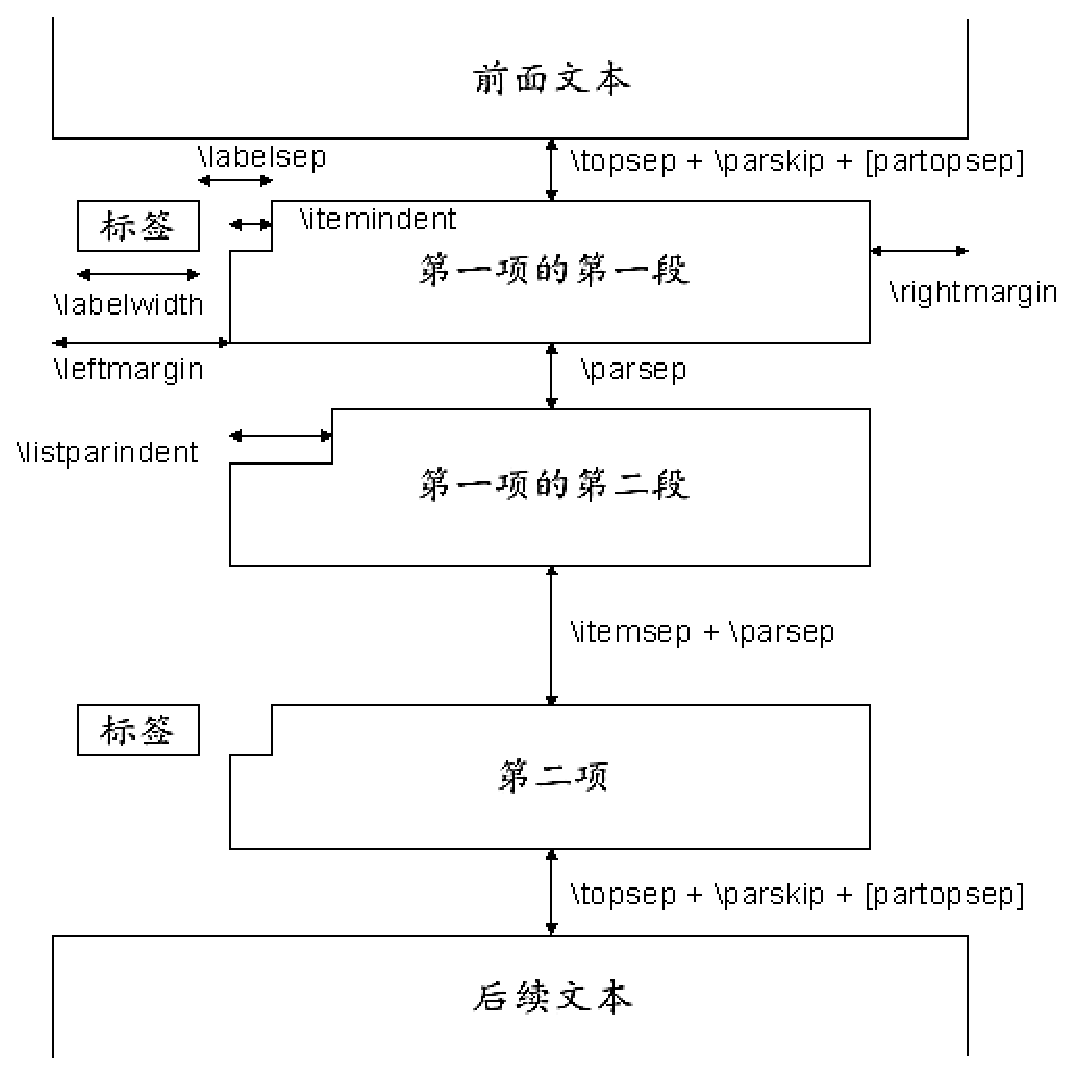
\includegraphics[width = 0.6\textwidth]{list}
\bicaption[list]{}{罗列环境参数示意图}{Fig.$\!$}{Schematic diagram of list environments}\vspace{-1em}
\end{figure}

通过调用~enumitem~宏包可以很方便地控制罗列环境的布局,其~format.tex~文件中的~\verb|\setitemize|~和~\verb|\setenumerate|~命令分别用来设置~\verb|itemize|~和~\verb|enumerate|~环境的样式参数。采用~\verb|itemize|~单层罗列环境的排版形式如下:

\begin{itemize}
\item 第一个条目文本内容
\item 第二个条目文本内容
\item 第三个条目文本内容
\end{itemize}

其代码如下
\begin{verbatim}
\begin{itemize}
  \item 第一个条目文本内容
  \item 第二个条目文本内容
  ...
  \item 第三个条目文本内容
\end{itemize}
\end{verbatim}

采用~\verb|enumerate|~单层罗列环境的排版形式如下:
\begin{enumerate}
\item 第一个条目文本内容
\item 第二个条目文本内容
\item 第三个条目文本内容
\end{enumerate}

其代码如下
\begin{verbatim}
\begin{enumerate}
  \item 第一个条目文本内容
  \item 第二个条目文本内容
  ...
  \item 第三个条目文本内容
\end{enumerate}
\end{verbatim}

例如:

\begin{enumerate}
\item 鉴定袋蛾———二十分
\item 给斯拉瓦写信———二小时四十五分
\item 植物保护小组开会———二小时二十五分
\end{enumerate}

上述是默认的列表样式。源代码如下:
\begin{lstlisting}
  \begin{enumerate}
  \item 鉴定袋蛾———二十分
  \item 给斯拉瓦写信———二小时四十五分
  \item 植物保护小组开会———二小时二十五分
  \end{enumerate}
\end{lstlisting}

\texttt{emumerate}环境就是罗列环境。每条\verb|\item| 后面
跟一个空格,然后就是具体的罗列条目。

默认的样式是按照1.、2.、3.、……来排序的,如果想按照英文字母(a),(b),(c)或者罗
马数字(i),(ii),(iii)这样的顺序呢,只需要
在 \verb|\item[]| 后面[~]中加入指定的序号。比如:
\begin{enumerate}
\item[(1)] 鉴定袋蛾———二十分
\item[(2)] 给斯拉瓦写信———二小时四十五分
\item[(3)] 植物保护小组开会———二小时二十五分
\end{enumerate}
源代码是:
\begin{lstlisting}
  \begin{enumerate}
  \item[(1)] 鉴定袋蛾———二十分
  \item[(2)] 给斯拉瓦写信———二小时四十五分
  \item[(3)] 植物保护小组开会———二小时二十五分
  \end{enumerate}
\end{lstlisting}

\section*{本章小结}[Brief Summary]
表格和罗列排版方法介绍。
